\begin{spacing}{1}
    \chapter*{Abstract [L]}
\end{spacing}
\begin{wrapfigure}{r}{0.3\textwidth}
    \begin{center}
      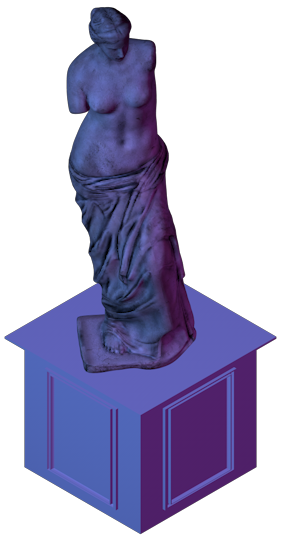
\includegraphics[width=0.2\textwidth]{pics/statue.png}
    \end{center}
\end{wrapfigure}
\setauthor{Litzlbauer Lorenz}
3D Portfolio Gallery is a web application developed by Lorenz Litzlbauer and Fabian Maar as part of the thesis. The 3D Portfolio Gallery aims to enable designers to share their design portfolio with the world in an innovative way, all in a virtual three-dimensional space. Designers can use 3D Portfolio Gallery to create a three-dimensional portfolio from their own media (film, photo or 3D data).
The 3D Portfolio Gallery is offered as a SPA on the web and can be accessed via a web link.
The 3D Portfolio Gallery provides a simple configuration process by selecting a gallery from several pre-defined layouts. In another step, the exhibition pieces are either automatically or manually placed and provided with additional information.

For the implementation in the front end, the following frameworks are used: Angular for the SPA (single-page application) and ThreeJs for the 3D presentation. The front-end access control and user identification in the browser uses JWT (JsonWebToken). The JWT is part of a standard described by the IETF III \href{https://www.rfc-editor.org/ rfc/rFc7519}{RFC7520}.
The backend uses Quarks as a server platform, Maven as a build system, and in the database access layer JPA (Java Persistence Architecture), Panach and Hibernate ORM.
\newpage
\begin{spacing}{1}
    \chapter*{Zusammenfassung [L]}
\end{spacing}
\begin{wrapfigure}{r}{0.3\textwidth}
    \begin{center}
      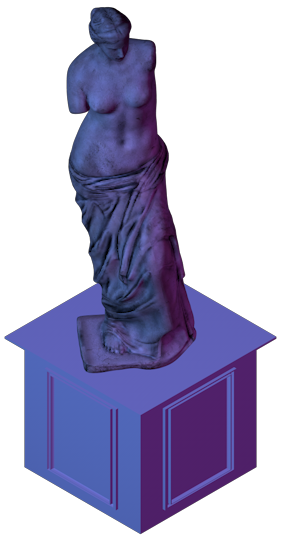
\includegraphics[width=0.2\textwidth]{pics/statue.png}
    \end{center}
\end{wrapfigure}
\setauthor{Litzlbauer Lorenz}
3D Portfolio Gallery ist eine Webapplikation, Lorenz Litzlbauer und Fabian Maar im Rahmen der Diplomarbeit entwickelt wurde. 3D Portfolio Gallery will Designer*innen ermöglichen, ihr Design-Portfolio auf eine innovative Art und Weise mit der Welt zu teilen und das alles in einem virtuellen dreidimensionalen Raum. Die Designer*innen können mithilfe von 3D Portfolio Gallery aus eigenen Medien (Film, Foto oder 3D-Daten) ein dreidimensionales Portfolio erstellen.
3D Portfolio Gallery wird als eine SPA im Web angeboten und ist über einen Web-Link erreichbar.
3D Portfolio Gallery bietet dafür einen einfachen Konfigurationsprozess, indem aus mehreren vordefinierten Grundrissen eine Gallery ausgewählt wird. In einem weiteren Schritt werden die Ausstellungsstücke entweder automatisch oder manuell platziert und mit Zusatzinformationen versehen.


Für die Umsetzung im Frontend werden folgende Frameworks verwendet: Angular für die SPA (Single-Page-Applikation) und ThreeJs für die 3D-Darstellung. . In der Frontend-Zugriffkontrolle und -Useridentifikation im Browser wird JWT (JsonWebToken) verwendet. Das JWT ist Teil eines Standards, der durch die III \href{https://www.rfc-editor.org/rfc/rfc7519}{RFC7519} IETF beschrieben wird.
Das Backend verwendet als Serverplattform Quarks, als Buildsystem Maven und in der Datenbankzugriffschicht JPA (Java Persistence Architecture), Panach und Hibernate ORM.
